%%%%%%%%%%%%%%%%%%%%%%%%%%%%%%%%%%%%%%%%%
% a0poster Portrait Poster
% LaTeX Template
% Version 1.0 (22/06/13)
%
% The a0poster class was created by:
% Gerlinde Kettl and Matthias Weiser (tex@kettl.de)
% 
% This template has been downloaded from:
% http://www.LaTeXTemplates.com
%
% License:
% CC BY-NC-SA 3.0 (http://creativecommons.org/licenses/by-nc-sa/3.0/)
%
%%%%%%%%%%%%%%%%%%%%%%%%%%%%%%%%%%%%%%%%%

%----------------------------------------------------------------------------------------
%	PACKAGES AND OTHER DOCUMENT CONFIGURATIONS
%----------------------------------------------------------------------------------------

\documentclass[a0,portrait]{a0poster}

\usepackage{multicol} % This is so we can have multiple columns of text side-by-side
\columnsep=100pt % This is the amount of white space between the columns in the poster
\columnseprule=3pt % This is the thickness of the black line between the columns in the poster

\usepackage[svgnames]{xcolor} % Specify colors by their 'svgnames', for a full list of all colors available see here: http://www.latextemplates.com/svgnames-colors

\usepackage{times} % Use the times font
%\usepackage{palatino} % Uncomment to use the Palatino font

\usepackage{graphicx} % Required for including images
\graphicspath{{figures/}} % Location of the graphics files
\usepackage{booktabs} % Top and bottom rules for table
\usepackage[font=small,labelfont=bf]{caption} % Required for specifying captions to tables and figures
\usepackage{amsfonts, amsmath, amsthm, amssymb} % For math fonts, symbols and environments
\usepackage{wrapfig} % Allows wrapping text around tables and figures
\usepackage[utf8]{inputenc}

\begin{document}

%----------------------------------------------------------------------------------------
%	POSTER HEADER 
%----------------------------------------------------------------------------------------

% The header is divided into two boxes:
% The first is 75% wide and houses the title, subtitle, names, university/organization and contact information
% The second is 25% wide and houses a logo for your university/organization or a photo of you
% The widths of these boxes can be easily edited to accommodate your content as you see fit

\begin{minipage}[b]{0.723\linewidth}
\veryHuge \color{NavyBlue} \textbf{Estimating pooled within-time series variograms with spatially shifted temporal points} \color{Black}\\[2cm]% Title
%\Huge\textit{An Exploration of Complexity}\\[2cm] % Subtitle
\huge \textbf{Avit Kumar Bhowmik\textsuperscript{1} and Pedro Cabral\textsuperscript{2}}\\[0.5cm] % Author(s)
\LARGE \textsuperscript{1}Institute for Environmental Sciences, University of Koblenz-Landau, Germany\\
\LARGE \textsuperscript{2}NOVA Information Management School, Universidade Nova de Lisboa, Portugal\\[0.4cm] % University/organization
\Large \texttt{bhowmik@uni-landau.de, https://github.com/AvitBhowmik/SSTP}\\
\end{minipage}
%
\begin{minipage}[b]{0.277\linewidth}

\includegraphics[width=20cm]{logo.png}\\
\end{minipage}

\vspace{1cm} % A bit of extra whitespace between the header and poster content

%----------------------------------------------------------------------------------------

\begin{multicols}{2} % This is how many columns your poster will be broken into, a portrait poster is generally split into 2 columns

%----------------------------------------------------------------------------------------
%	ABSTRACT
%----------------------------------------------------------------------------------------

%\color{Navy} % Navy color for the abstract

%\begin{abstract}

%We developed an alternative method, i.e. spatially shifting temporal points (SSTP), for pooled within-time series (PTS) variogram estimation using R open-source software environment. The method spatializes temporal data points by shifting them to arbitrary coordinate clusters, and a PTS variogram is estimated by controlling lower and upper boundaries of spatial-lags. We applied SSTP for PTS variogram estimation of a precipitation index in a data-scarce region. SSTP exhibited higher precision than the available method of averaging semivariances over spatial-lags. 

%\end{abstract}

%----------------------------------------------------------------------------------------
%	INTRODUCTION
%----------------------------------------------------------------------------------------

\color{SaddleBrown} % SaddleBrown color for the introduction

\section*{Introduction}

Estimation of pooled within-time series (PTS) variograms is frequently done for geostatistical interpolation in spatially data-scarce regions \cite{wagner_comparison_2012}. The only available averaging empirical variograms (AEV) method averages semivariances that are computed for individual time steps over each spatial-lag within a pooled time series \cite{graler_spatio-temporal_2011}. However, semivariances computed by a few paired comparisons in individual time steps are erratic and hence hamper precision of PTS variogram estimation.

Here, we outline an alternative method, i.e. ``spatially shifting temporal points (SSTP)'', for PTS variogram estimation that was developed using R open source software environment.
%----------------------------------------------------------------------------------------
%	OBJECTIVES
%----------------------------------------------------------------------------------------

\color{DarkSlateGray} % DarkSlateGray color for the rest of the content

%\section*{Main Objectives}

%\begin{enumerate}
%\item Lorem ipsum dolor sit amet, consectetur.
%\item Nullam at mi nisl. Vestibulum est purus, ultricies cursus volutpat sit amet, vestibulum eu.
%\item Praesent tortor libero, vulputate quis elementum a, iaculis.
%\item Phasellus a quam mauris, non varius mauris. Fusce tristique, enim tempor varius porta, elit purus commodo velit, pretium mattis ligula nisl nec ante.
%\item Ut adipiscing accumsan sapien, sit amet pretium.
%\item Estibulum est purus, ultricies cursus volutpat
%\item Nullam at mi nisl. Vestibulum est purus, ultricies cursus volutpat sit amet, vestibulum eu.
%\item Praesent tortor libero, vulputate quis elementum a, iaculis.
%\end{enumerate}

%----------------------------------------------------------------------------------------
%	MATERIALS AND METHODS
%----------------------------------------------------------------------------------------

\section*{Methods}

\subsection*{Spatially shifting temporal points}

The temporal data point sets were spatialized, i.e. assigned to different coordinate clusters on the same space (Figure 1 and 2). $s$ is a data point location vector with coordinate touples $(x,y)$, $t$ is a time vector, $Z(s,t)$ is the vector for a random process in data point $s$ and year $t$, $||s_{i,t}-s_{j,t}||$ is the spatial-lag for the point pair $s_i$ and $s_j$ in year $t$; $i,j \in 1..n$. We first assigned the points from $t_1$ to its original coordinates $x_{t_1},y_{t_1}$. The coordinates for the the latter years were calculated according to Eq. (1), when $(t_1+1)+4n \leq t<(t_1+1)+4(n+1)$; $n \in N$.

\begin{equation}
\begin{split}
s_{(t_1+1)+4n} = x_{(t_1+1)+4n}+(n+1)d, y_{(t_1+1)+4n} \\
s_{(t_1+1)+4n+1} = x_{(t_1+1)+4n+1}-(n+1)d, y_{(t_1+1)+4n+1} \\
s_{(t_1+1)+4n+2} = x_{(t_1+1)+4n+2}, y_{(t_1+1)+4n+2}+(n+1)d \\
s_{(t_1+1)+4n+3} = x_{(t_1+1)+4n+3}, y_{(t_1+1)+4n+3}-(n+1)d \\ \\
where, d>2(max||s_{i,t}-s_{j,t}||)
\end{split}
\end{equation}

\begin{center}
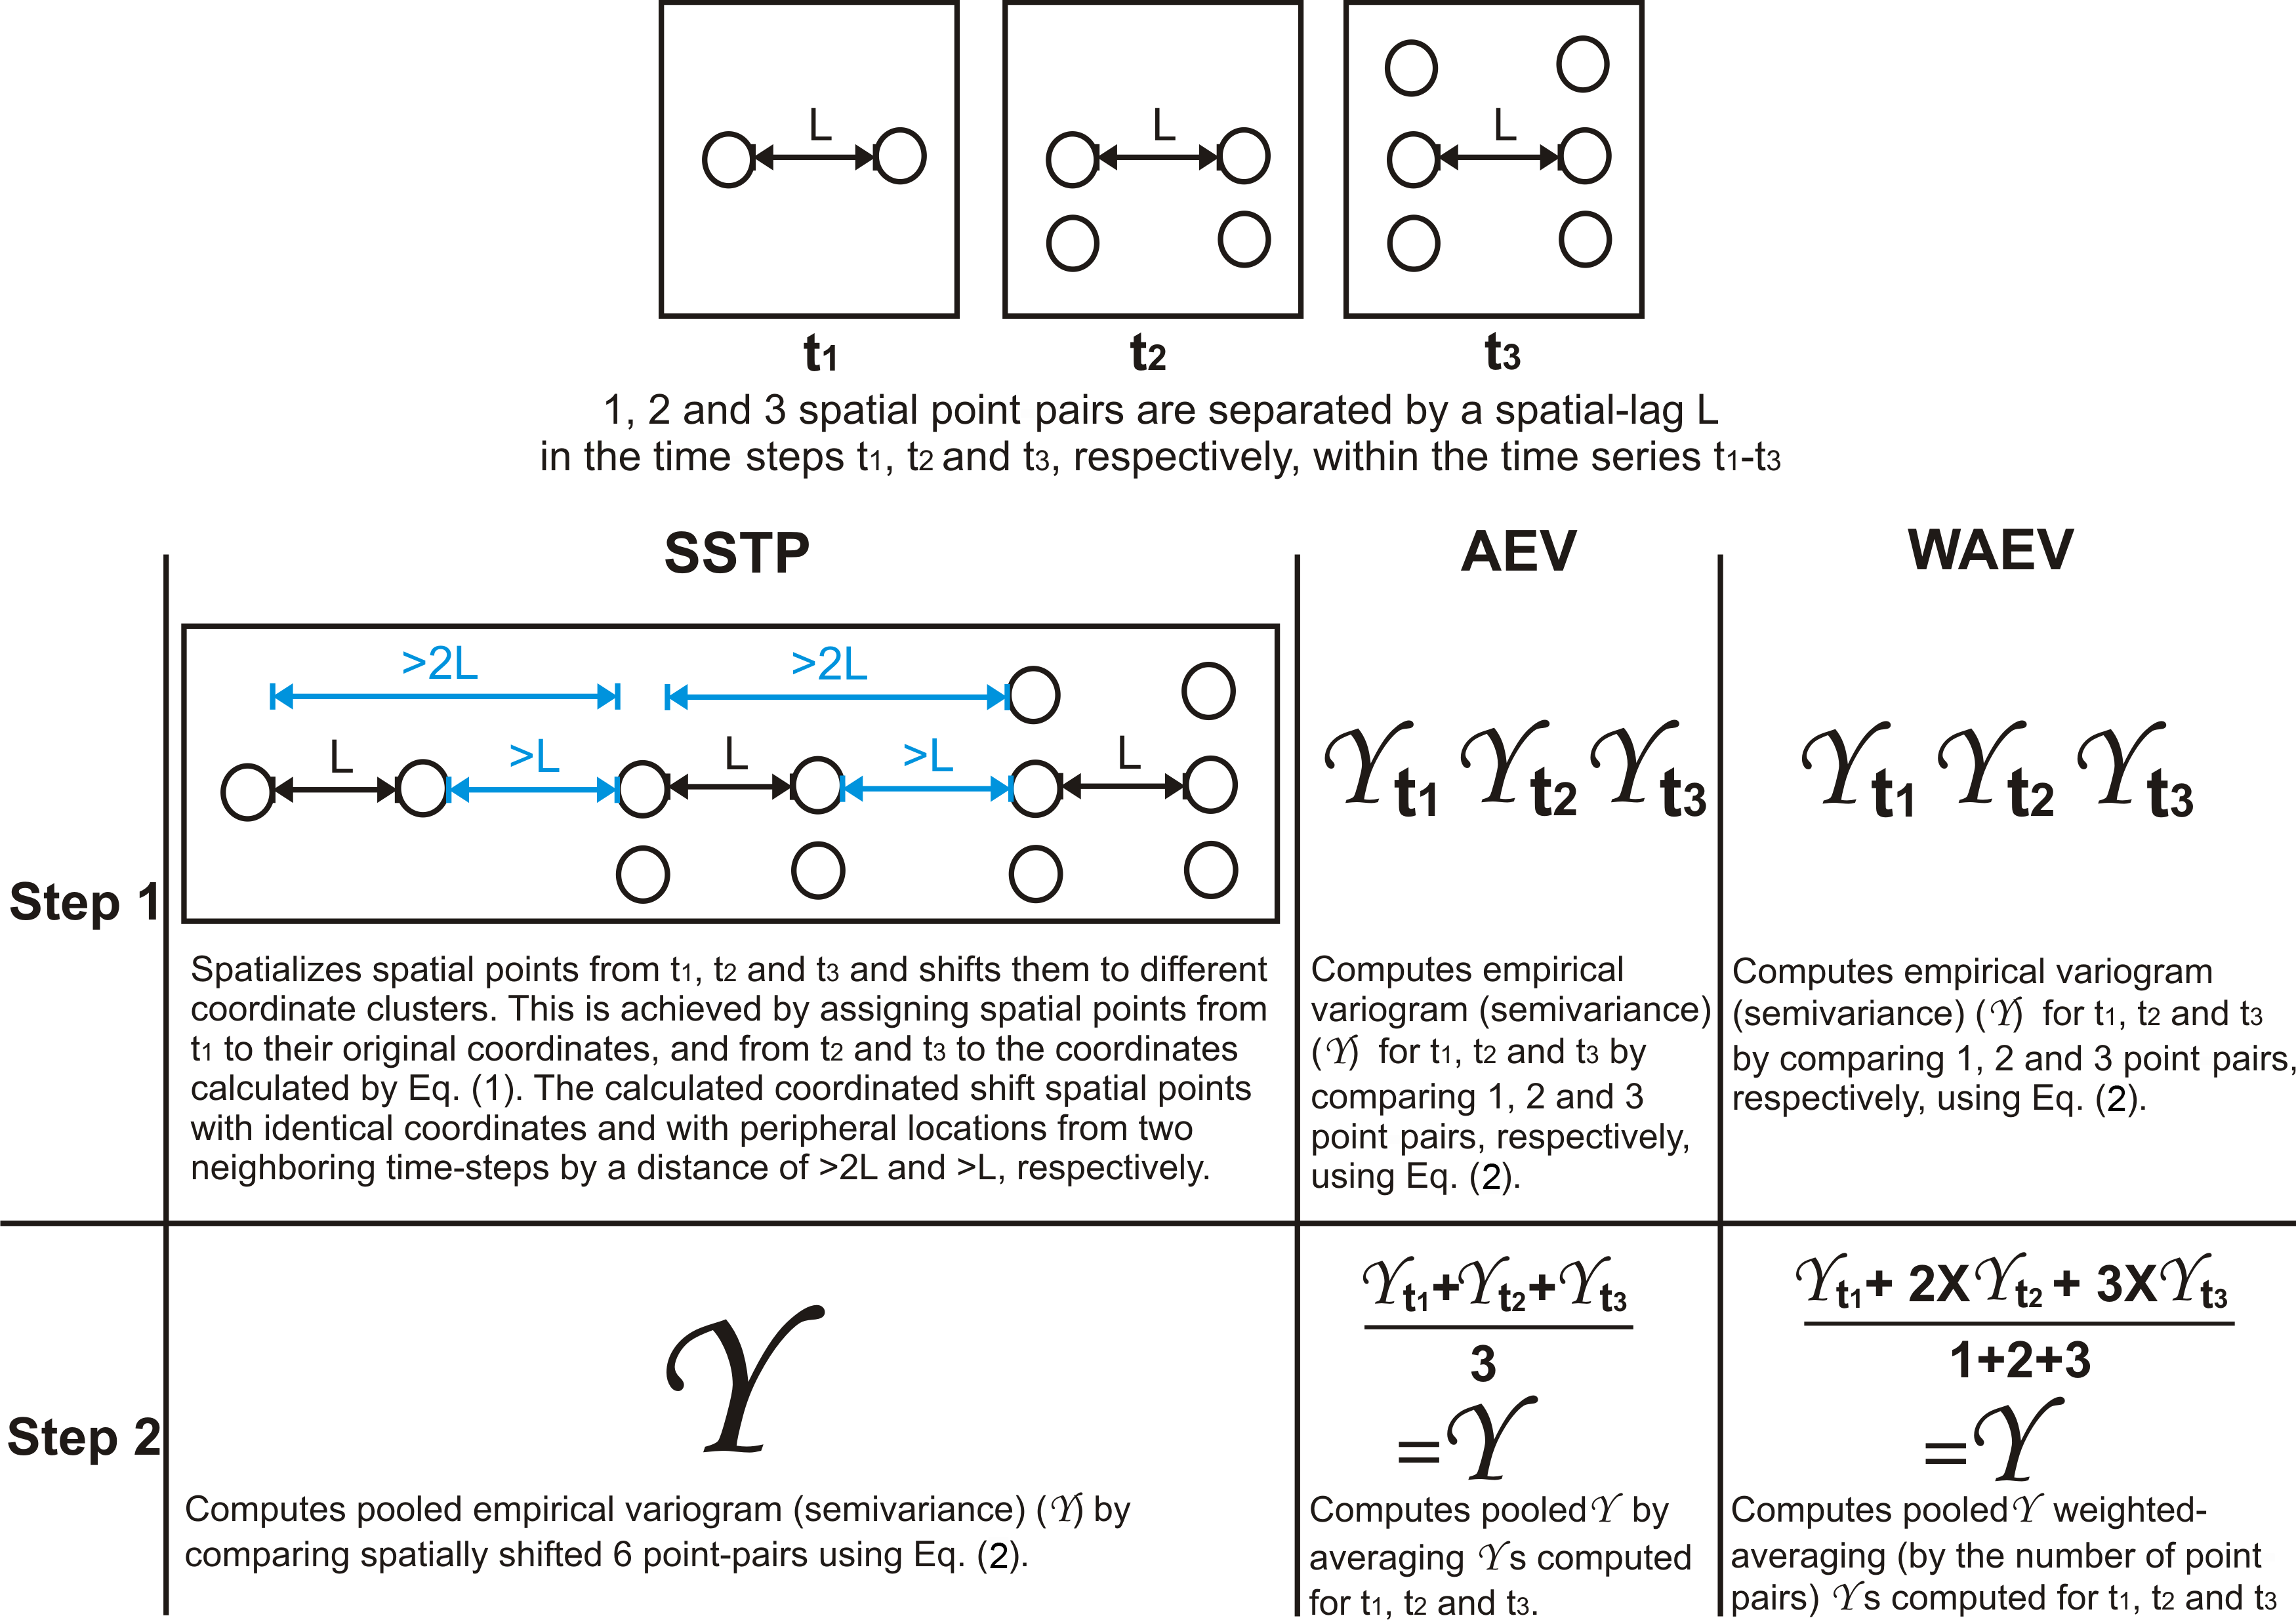
\includegraphics[width=1\linewidth]{Fig_1}
\captionof{figure}{\color{Green} Work-flows of spatially shifting temporal points (SSTP), averaging empirical variograms (AEV) and weighted AEV methods.}
\end{center}

\subsection*{Estimation of pooled within-time series variograms}

The empirical variograms were computed by simulatenous comparison of spatially shifted points using the commonly applied Methods of Moments (MoM) \cite{webster_geostatistics_2007}. For the point pair $s_i$ and $s_j$, the pooled semivariance $\gamma ||s_i-s_j||$ was computed by Eq. (2).

\begin{equation}
\begin{split}
\gamma ||s_i-s_j||=\frac{1}{2M||s_i-s_j||}\sum_{i,j}(Z(s_i)-Z(s_j))^2 \\ \\
where, ||s_1-s_2||=min||s_{i,t}-s_{j,t}||; ||s_{n-1}-s_n||=max||s_{i,t}-s{j,t}||
\end{split}
\end{equation}

We checked for anisotropy and computed the ratio between the major and minor axes ($A:B$) of the anisotropy ellipse and the anisotropy angle ($\phi$).

The available variogram models were fitted to the computed semivariances by a weighted least square approach providing $\frac{M||s_i-s_j||}{(s_i-s_j)^2}$ as weights. The nugget, partial sill, and range ($a$) parameters were extracted.

Precision of the PTS variogram estimation was evaluated by (i) variogram model-fit (weighted mean of squared error (MSE)) and (ii) cross-validation of a universal kriging (UK) interpolation (root means squared error (RMSE) and Nash-Sutcliffe efficiency (NSE)) using the best-fit models.

%\subsection*{Pooling time series}
\subsection*{Study area and data}

SSTP was applied to the PTS variogram estimation for ``annual total precipitation in hydrological wet days (PRCPTOT)'' in Bangladesh (Figure 2). Currently, 32 rain-gauges report daily precipitation in Bangladesh, classifying the country as data scarce. Moreover, the numbers of data points exhibit an increasing coverage from 8 in 1948 to 32 in 2007, indicating variable lengths of the time-series. PTS variograms were also estimated using the available AEV and weighted AEV (WAEV) (see Figure 1 for details) and the precision statistics were compared with the SSTP estimated variograms.

\begin{center}
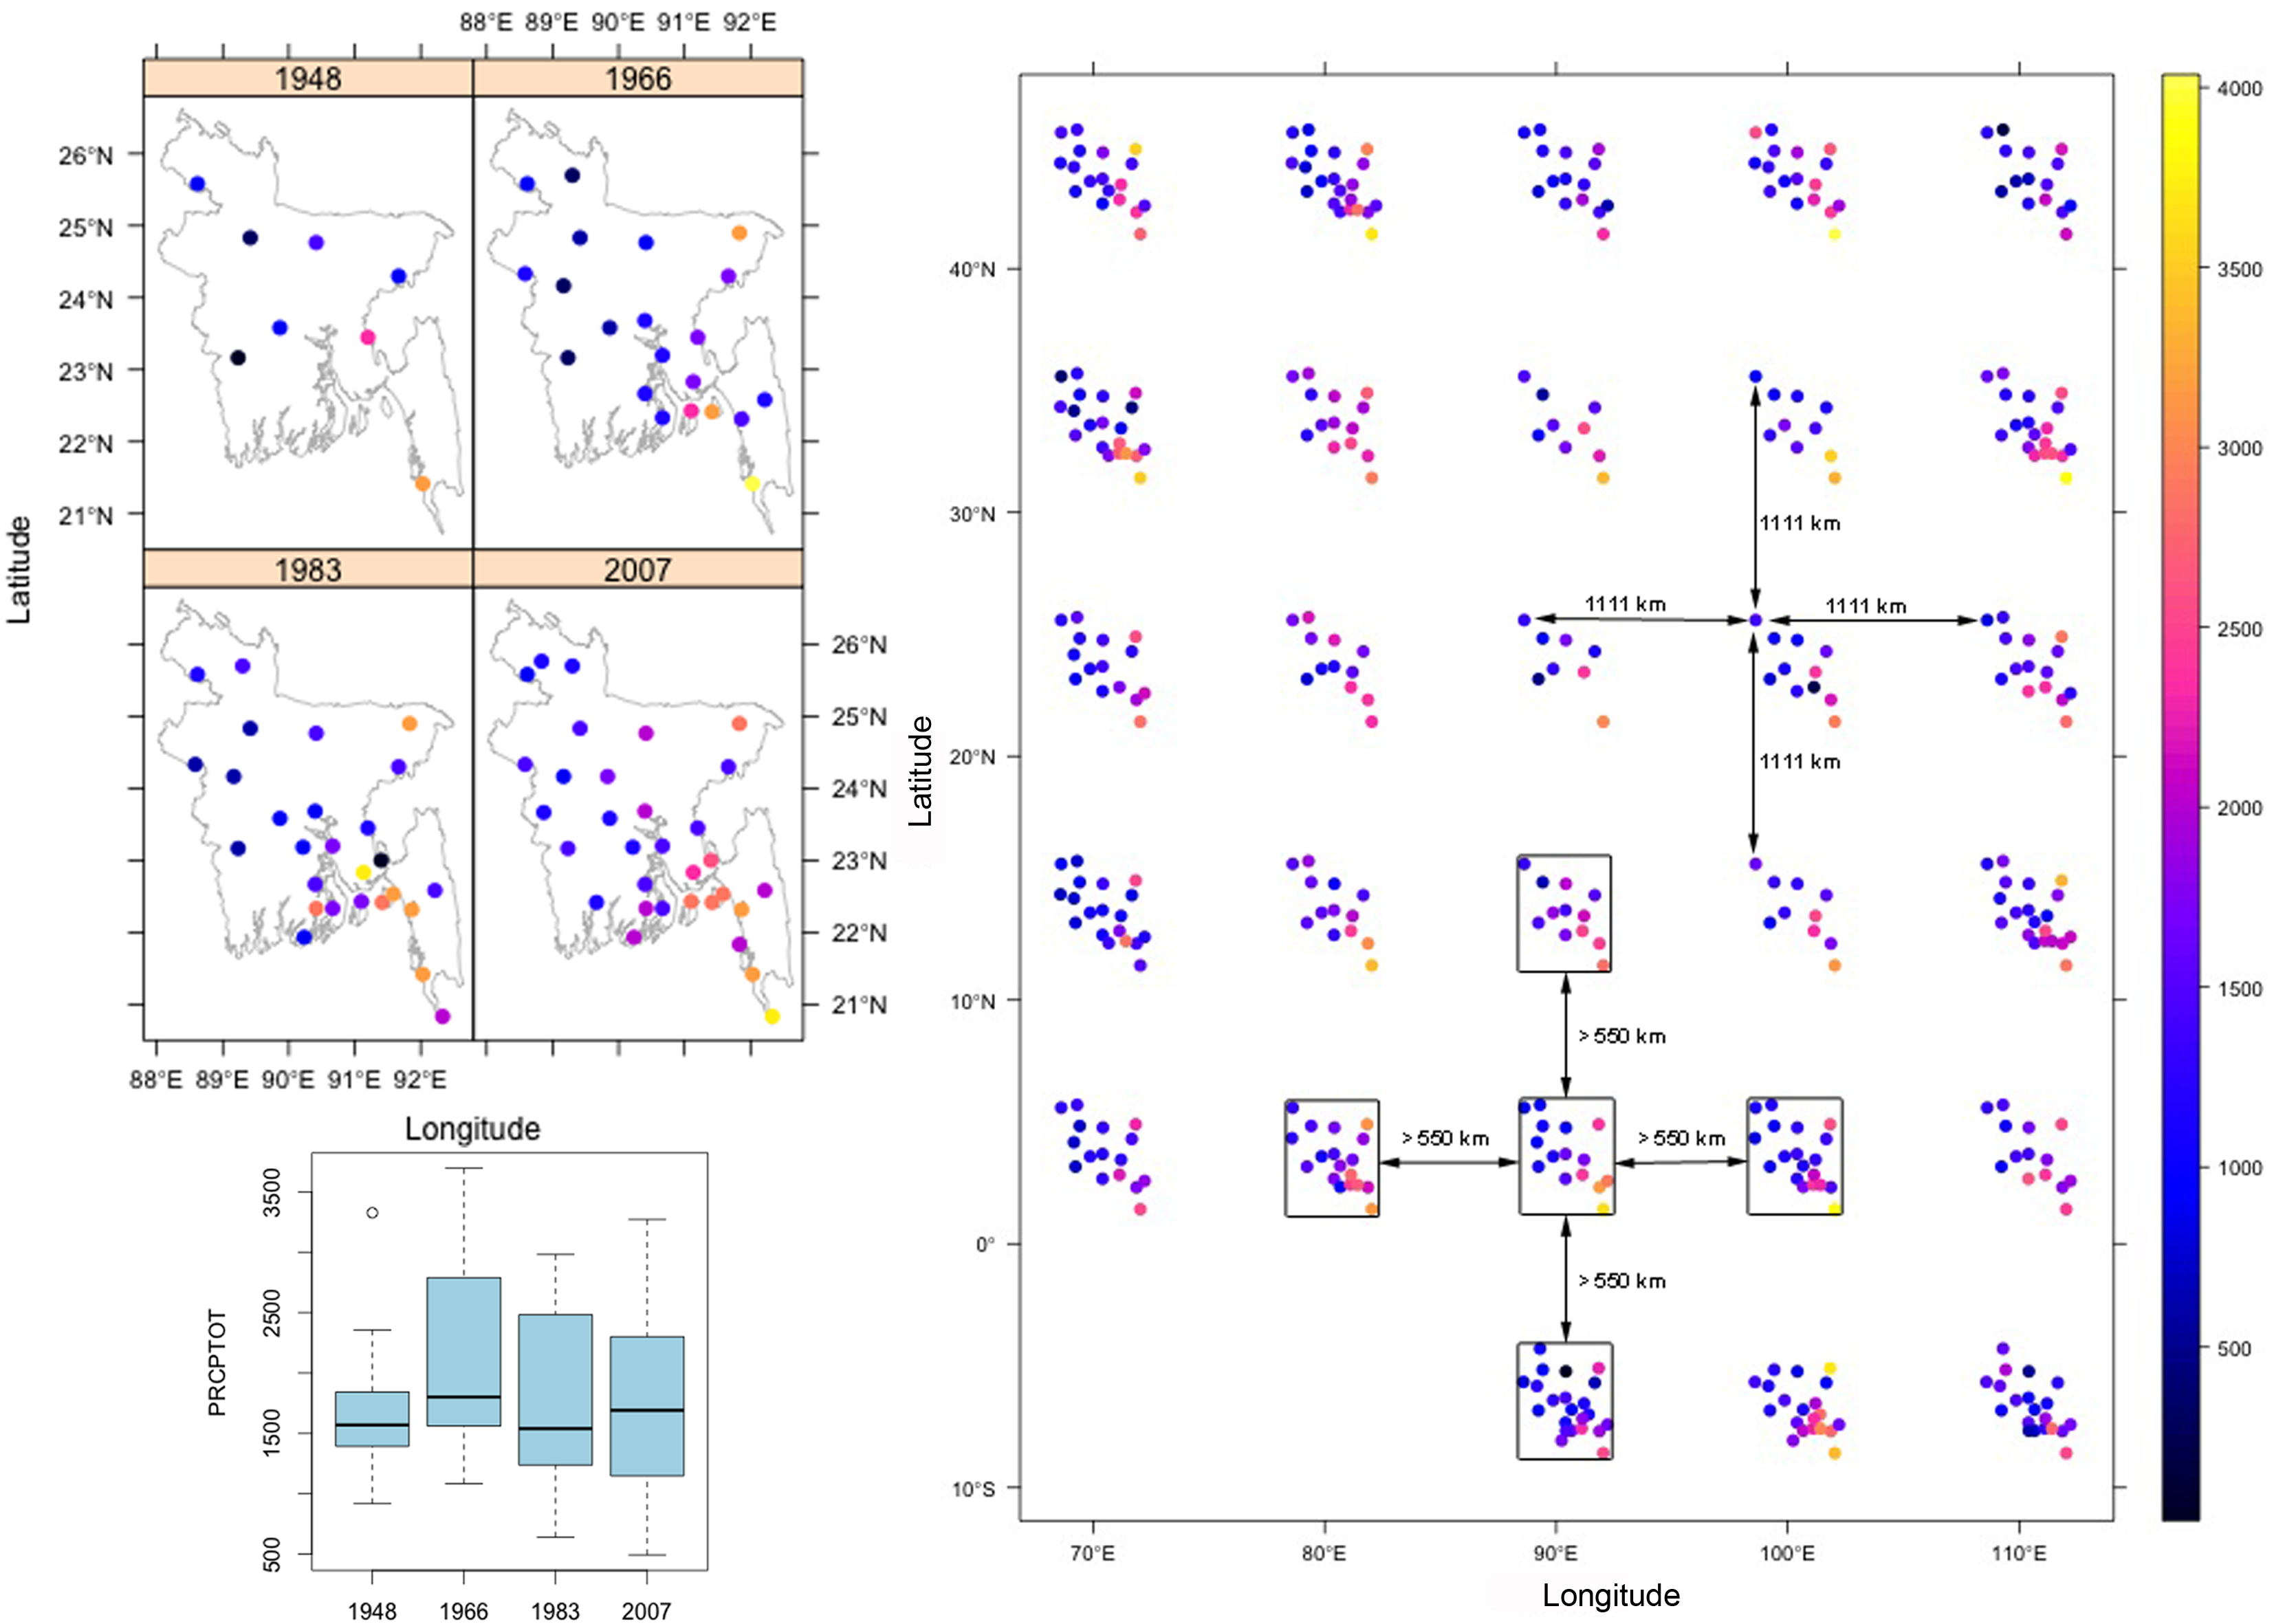
\includegraphics[width=1\linewidth]{Fig_2}
\captionof{figure}{\color{Green} PRCPTOT points \& distribution in four representative years (left) and SSTP for 1948-1975 series (right).}
\end{center} 

%We first quantified spatial structure in the data by computing its spatial correlation coefficients along the longitudinal and latitudinal gradients and then applied the Pettitt–Mann–Whitney test to the correlation coefficients to identify changes within a time series. The (sub)time series between the change points were extracted as time series with consistent spatial structure. Next, we checked for the stationarity within the extracted time series by applying the Augmented Dickey-Fuller test. Finally, the time series with consistent spatial structure and stationarity were checked to ensure that the numbers of pooled data points meet the threshold for reliable variogram estimation.
%------------------------------------------------

%\subsection*{Mathematical Section}

%Nulla vel nisl sed mauris auctor mollis non sed.

%\begin{equation}
%E = mc^{2}
%\label{eqn:Einstein}
%\end{equation}

%Curabitur mi sem, pulvinar quis aliquam rutrum. (1) edf (2)
%, $\Omega=[-1,1]^3$, maecenas leo est, ornare at. $z=-1$ edf $z=1$ sed interdum felis dapibus sem. $x$ set $y$ ytruem. 
%Turpis $j$ amet accumsan enim $y$-lacina; 
%ref $k$-viverra nec porttitor $x$-lacina. 

%Vestibulum ac diam a odio tempus congue. Vivamus id enim nisi:

%\begin{eqnarray}
%\cos\bar{\phi}_k Q_{j,k+1,t} + Q_{j,k+1,x}+\frac{\sin^2\bar{\phi}_k}{T\cos\bar{\phi}_k} Q_{j,k+1} &=&\nonumber\\ 
%-\cos\phi_k Q_{j,k,t} + Q_{j,k,x}-\frac{\sin^2\phi_k}{T\cos\phi_k} Q_{j,k}\label{edgek}
%\end{eqnarray}
%and
%\begin{eqnarray}
%\cos\bar{\phi}_j Q_{j+1,k,t} + Q_{j+1,k,y}+\frac{\sin^2\bar{\phi}_j}{T\cos\bar{\phi}_j} Q_{j+1,k}&=&\nonumber \\
%-\cos\phi_j Q_{j,k,t} + Q_{j,k,y}-\frac{\sin^2\phi_j}{T\cos\phi_j} Q_{j,k}.\label{edgej}
%\end{eqnarray} 

%Nulla sed arcu arcu. Duis et ante gravida orci venenatis tincidunt. Fusce vitae lacinia metus. Pellentesque habitant morbi. $\mathbf{A}\underline{\xi}=\underline{\beta}$ Vim $\underline{\xi}$ enum nidi $3(P+2)^{2}$ lacina. Id feugain $\mathbf{A}$ nun quis; magno.

%----------------------------------------------------------------------------------------
%	RESULTS 
%----------------------------------------------------------------------------------------
\color{SaddleBrown} % SaddleBrown color for the conclusions to make them stand out

\section*{Results and Conclusion}

``Power model'' showed the best-fit for all methods and pooled series except for SSTP in 1948-2007. SSTP computed semivariances exhibited much less noise than the AEV and WAEV, and consequently PTS variograms estimated by SSTP showed lower MSE and RMSE, and higher NSE indicating higher precision than AEV and WAEV (Figure 3). SSTP reduces uncertainty for variogram modelling while preserving spatiotemporal properties. It can be improved by including temporal autocorrelation, external variables and expert elicitation.
%
%\begin{wraptable}{l}{12cm} % Left or right alignment is specified in the first bracket, the width of the table is in the second
%\begin{tabular}{l l l}
%\toprule
%\textbf{Treatments} & \textbf{Response 1} & \textbf{Response 2}\\
%\midrule
%Treatment 1 & 0.0003262 & 0.562 \\
%Treatment 2 & 0.0015681 & 0.910 \\
%Treatment 3 & 0.0009271 & 0.296 \\
%\bottomrule
%\end{tabular}
%\captionof{table}{\color{Green} Table caption}
%\end{wraptable}
%
%Phasellus imperdiet, tortor vitae congue bibendum, felis enim sagittis lorem, et volutpat ante orci sagittis mi. Morbi rutrum laoreet semper. Morbi accumsan enim nec tortor consectetur non commodo nisi sollicitudin. Proin sollicitudin. Pellentesque eget orci eros. Fusce ultricies, tellus et pellentesque fringilla, ante massa luctus libero, quis tristique purus urna nec nibh.

%Nulla ut porttitor enim. Suspendisse venenatis dui eget eros gravida tempor. Mauris feugiat elit et augue placerat ultrices. Morbi accumsan enim nec tortor consectetur non commodo. Pellentesque condimentum dui. Etiam sagittis purus non tellus tempor volutpat. Donec et dui non massa tristique adipiscing. Quisque vestibulum eros eu. Phasellus imperdiet, tortor vitae congue bibendum, felis enim sagittis lorem, et volutpat ante orci sagittis mi. Morbi rutrum laoreet semper. Morbi accumsan enim nec tortor consectetur non commodo nisi sollicitudin.

\begin{center}
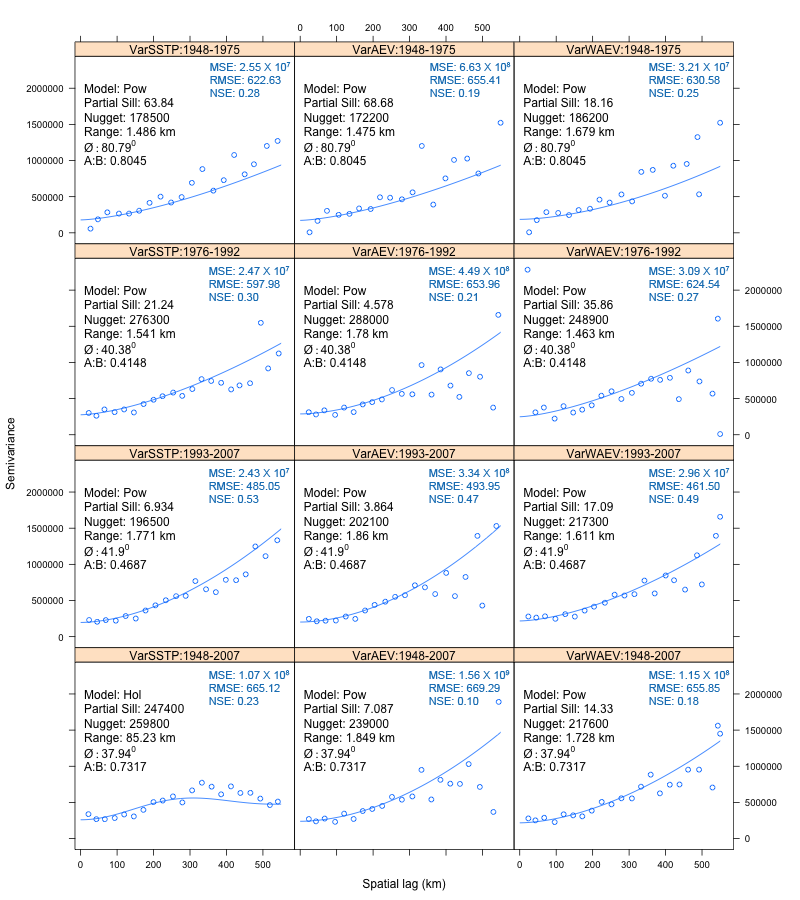
\includegraphics[width=1\linewidth]{Fig_3}
\captionof{figure}{\color{Green} Estimated PTS variograms by SSTP, AEV and WAEV methods with model parameters and precision statistics.}
\end{center}

%\begin{center}\vspace{1cm}
%\begin{tabular}{l l l l}
%\toprule
%\textbf{Treatments} & \textbf{Response 1} & \textbf{Response 2} \\
%\midrule
%Treatment 1 & 0.0003262 & 0.562 \\
%Treatment 2 & 0.0015681 & 0.910 \\
%Treatment 3 & 0.0009271 & 0.296 \\
%\bottomrule
%\end{tabular}
%\captionof{table}{\color{Green} Table caption}
%\end{center}\vspace{1cm}

%Vivamus sed nibh ac metus tristique tristique a vitae ante. Sed lobortis mi ut arcu fringilla et adipiscing ligula rutrum. Aenean turpis velit, placerat eget tincidunt nec, ornare in nisl. In placerat.

%----------------------------------------------------------------------------------------
%	CONCLUSIONS
%----------------------------------------------------------------------------------------

%\color{SaddleBrown} % SaddleBrown color for the conclusions to make them stand out

%\section*{Conclusions}

%\begin{itemize}
%\item Pellentesque eget orci eros. Fusce ultricies, tellus et pellentesque fringilla, ante massa luctus libero, quis tristique purus urna nec nibh. Phasellus fermentum rutrum elementum. Nam quis justo lectus.
%\item Vestibulum sem ante, hendrerit a gravida ac, blandit quis magna.
%\item Donec sem metus, facilisis at condimentum eget, vehicula ut massa. Morbi consequat, diam sed convallis tincidunt, arcu nunc.
%\item Nunc at convallis urna. isus ante. Pellentesque condimentum dui. Etiam sagittis purus non tellus tempor volutpat. Donec et dui non massa tristique adipiscing.
%\end{itemize}

\color{DarkSlateGray} % Set the color back to DarkSlateGray for the rest of the content

%----------------------------------------------------------------------------------------
%	FORTHCOMING RESEARCH
%----------------------------------------------------------------------------------------

%\section*{Forthcoming Research}

%Vivamus molestie, risus tempor vehicula mattis, libero arcu volutpat purus, sed blandit sem nibh eget turpis. Maecenas rutrum dui blandit lorem vulputate gravida. Praesent venenatis mi vel lorem tempor at varius diam sagittis. Nam eu leo id turpis interdum luctus a sed augue. Nam tellus.

 %----------------------------------------------------------------------------------------
%	REFERENCES
%----------------------------------------------------------------------------------------

%\nocite{*} % Print all references regardless of whether they were cited in the poster or not
\bibliographystyle{unsrt} % Plain referencing style
\bibliography{SPAT_Bhowmik} % Use the example bibliography file sample.bib

%----------------------------------------------------------------------------------------
%	ACKNOWLEDGEMENTS
%----------------------------------------------------------------------------------------

%\section*{Acknowledgements}

%Etiam fermentum, arcu ut gravida fringilla, dolor arcu laoreet justo, ut imperdiet urna arcu a arcu. Donec nec ante a dui tempus consectetur. Cras nisi turpis, dapibus sit amet mattis sed, laoreet.

%----------------------------------------------------------------------------------------

\end{multicols}
\end{document}